Shared-memory parallelisation and comparison with MPI

\subsection{Shared-memory parallelisation}

MPI may be faster than GMCF but the GMCF performance is competitive. MPICH was
the initial implementation of the MPI 1.x standard so is around two decades old.
GMCF's implementation began in August 2014, less than a year ago and is
primarily aimed at model coupling, not parallelism. As GMCF matures it can be
expected that the performance gap will narrow.

\begin{figure}
    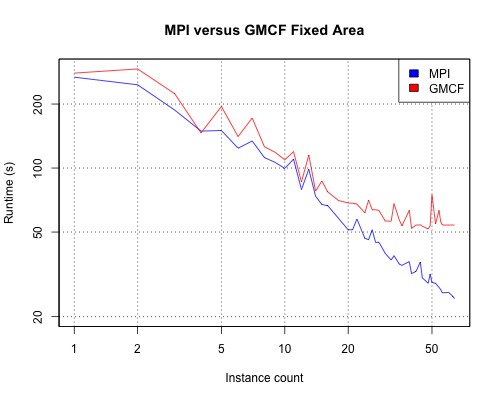
\includegraphics[width=0.5\textwidth]{graphs/GMCF-MPI-fixed-area}
    \caption{MPI versus GMCF Fixed Area}
    \label{fig:gmcfmpifixedarea}
\end{figure}

\begin{figure}
    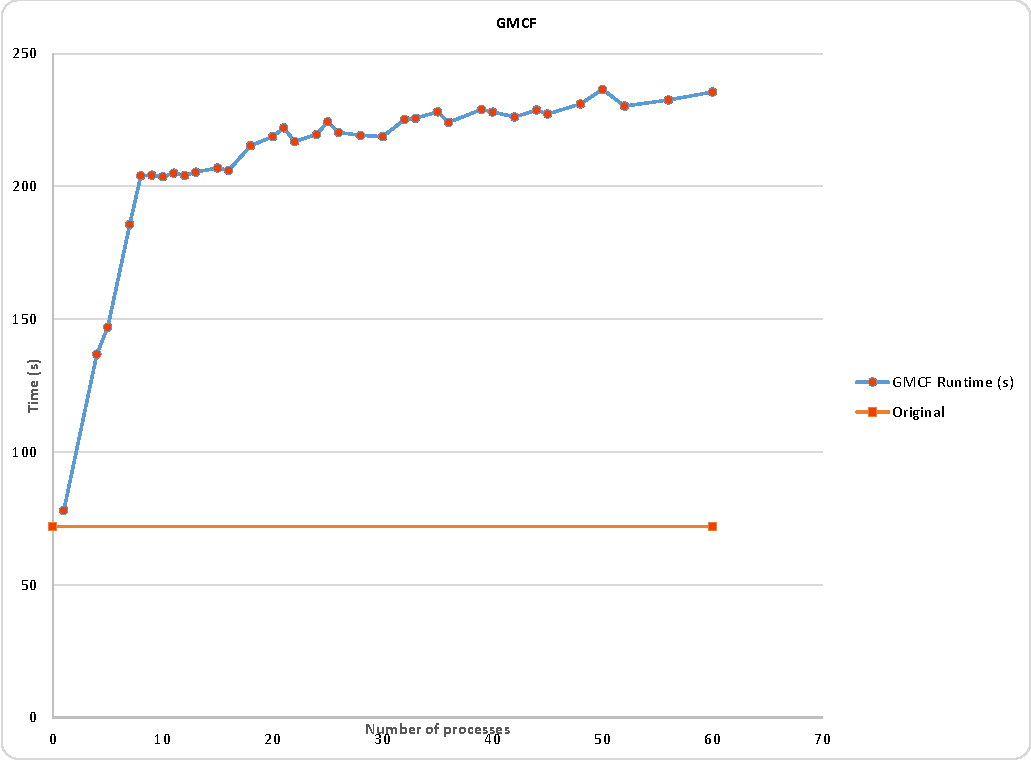
\includegraphics[page=1,width=0.5\textwidth]    {graphs/gmcfThreadPinningFasterSorNoREQDATAnewAPISpinBusyWaitExpandingArea-crop.pdf}
    \caption{GMCF Expanding Area}
    \label{fig:gmcfexpandingarea}
\end{figure}

Figure~\ref{fig:gmcfmpifixedarea} shows the performance scaling for a fixed
area. This scales up to 62 threads. 63 and 64 threads have poor performance
because there are two non-model threads in GMCF. These are also busy waiting
hence two cores are spent not doing model work. This is about 2.5x slower than
MPI but is still competitive.

Figure~\ref{fig:gmcfexpandingarea} shows the performance scaling for an
expanding area. The scaling situation is the same as for the fixed area version.
There is little difference in runtime between MPI and GMCF in this scenario.

\subsection{Comparison to MPI}

Figure~\ref{fig:gmcfmpifixedarea} shows that, for fixed area, MPI goes to around
25 seconds, GMCF goes to around 55 seconds.

Figure~\ref{fig:gmcfmpiexpandingarea} shows that, for expanding area, MPI goes
up to around 220 seconds, GMCF does the same but performance degrades quicker.
